\documentclass[english,serif,mathserif,xcolor=pdftex,dvipsnames,table]{beamer}
\usepackage{gc3}

\usepackage{graphicx}
\usepackage{alltt}
\usepackage{ulem}

\title[Introduction on GC3Pie]{%
  Introduction on GC3Pie
}
\author[Sergio Maffioletti]{%
  GC3: Grid Computing Competence Center, \\
  University of Zurich
}
\date{Oct.~1, 2012}

\begin{document}

% title frame
\maketitle

%% quick general intro to GC3Pie 15'
%%     purpose: toolkit for building "application control logic" in Python
%%     demo of a simple use case [ with video from ggamess ]
%%     links to documentation 

%% intro to GC3Pie programming 30'
%%     form: a library of Python object, mostly customized by inheritance ("Template method" pattern)
%%     GC3Pie execution model
%%     show steps of generic HTC script

\begin{frame}
  \begin{center}
    \huge{What is {\color{Blue} GC3Pie} and \\ why do we need something like that ?}
  \end{center}
\end{frame}

\begin{frame}
  \frametitle{high-throughput (HTC) use cases I}
  
  \begin{block}{}
    Run application on a {\color{Blue} range} of different inputs.
    Each input is a different file (or a set of files).
  \end{block}
    
  \begin{block}{}
    Then {\color{Blue} collect} output files and post-process them, e.g., gather some
    statistics.
  \end{block}

  \begin{block}{}
    Typically implemented by a set of \texttt{sh} / \texttt{perl} scripts to drive
    execution on a local cluster.
  \end{block}
\end{frame}

\begin{frame}
  \frametitle{high-throughput (HTC) use cases II}

  \begin{block}{}
    Need to {\color{Blue} chain together} different execution steps
    (workflow)
  \end{block}

  \begin{block}{}
    Execution flow is not {\color{Blue} uniform} (e.g. do not have to
    repeat the same action over every input)
  \end{block}

  \begin{block}{}
    Execution flow is determined at runtime ({\color{Blue} dynamic
    dependency})
  \end{block}

\end{frame}

\begin{frame}
  \frametitle{Potential issues}
  \begin{enumerate}
  \item \textbf{Portability:} Cannot run on a different cluster without
    rewriting all the scripts.
  \item \textbf{Code reuse:} Scripts are often very tied to a certain purpose, so
    they are difficult to reuse.
  \item \textbf{Heavy maintenance:} the more a script does its job well, the more
    you'll find yourself adding \texttt{generic} features and maintaining
    requests from other users.
  \end{enumerate}
\end{frame}

\begin{frame}
  \frametitle{Recurring patterns for an HTC driver script}
  \begin{enumerate}
  \item{\textbf{Access}} to computational resources
  \item{\textbf{Supervise}} execution of collection of jobs
  \item{\textbf{Handling}} of error conditions individually
  \item{\textbf{Post-process}} and store results
  \end{enumerate}
\end{frame}

\begin{frame}
\frametitle{What is GC3Pie ?}
  \begin{block}{}
    GC3Pie is a {\color{Blue} Python} toolkit:
  \end{block}

  \begin{block}{}
    it provides the building blocks to write Python scripts to run large {\color{Blue} computational campaigns} and 
  \end{block}

  \begin{block}{}
    to {\color{Blue} combine} several tasks into a dynamic
    {\color{Blue} workflow}.
  \end{block}
\end{frame}

\begin{frame}
\frametitle{What is GC3Pie ?}

  GC3Pie consists of three main components:
  
  \begin{block}{GC3Libs:} Python library for controlling the life-cycle of computational job collections. \end{block}
  \begin{block}{GC3Apps:} A collection of driver scripts to run large job campaigns. \end{block}
  \begin{block}{GC3Utils:} This is a small set of low-level utilities exposing the main functionality provided by GC3Libs. \end{block}
\end{frame}

\begin{frame}[fragile]
  \frametitle{An example: ggamess}
  \begin{alltt}
import gc3libs
from gc3libs.application.gamess 
     {\color{Blue}import} GamessApplication
from gc3libs.cmdline 
     {\color{Blue}import} SessionBasedScript

class {\color{Violet} GGamessScript}({\color{Violet}SessionBasedScript}):
  def \_\_init\_\_(self):
    SessionBasedScript.\_\_init\_\_(
       self,
       application = {\color{Violet}GamessApplication},
       input_filename_pattern = '{\color{Green}*.inp}'
    )
             
if \_\_name\_\_ == '{\color{Green}\_\_main\_\_}':
  GGamessScript().{\color{Blue}run()}
\end{alltt}
\end{frame}


%% \begin{frame}
%%   \frametitle{ggamess example}
%%   \begin{center}
%%     \large{The video...}
%%   \end{center}
%% \end{frame}

\begin{frame}
  \frametitle{GC3Pie for developers}
    \begin{block}{}
      Programming model based on customization of base classes through
      inheritance ({\color{Blue}Template method} pattern)
    \end{block}
    
    \begin{block}{}
      Different level of {\color{Blue}interfaces} depending on the control required
    \end{block}

    \begin{block}{}
      {\color{Blue}SessionBasedScript} is the highest level of abstraction
    \end{block}
\end{frame}

\begin{frame}
  \frametitle{How is GC3Pie different? (I)}
  
  \begin{block}{}
    GC3Pie runs specific \textbf{applications}, not generic jobs.
  \end{block}
  
   \begin{block}{}
     That is, GC3Pie exposes \texttt{Application} classes whose programming
    interface is adapted to the specific task/computation a scientific
    application performs.
  \end{block}
    
  \begin{block}{}
    You can add your own application by specializing the generic
    \texttt{Application} class.
  \end{block}
\end{frame}

\begin{frame}
  \frametitle{How is GC3Pie different? (II)}
  
  \begin{block}{}
    GC3Pie can run applications in parallel, or sequentially, or any
    combination of the two, and do arbitrary processing of data in the
    middle.
  \end{block}
  
  \begin{block}{}
    Think of {\color{Blue}workflows}, except you can write them in the Python
    programming language.
  \end{block}
  
  \begin{block}{}
    Which means, you can create them dynamically at runtime, adapting
    the schema to your problem.
  \end{block}
\end{frame}

\begin{frame}
  \frametitle{GC3Pie Execution model}
  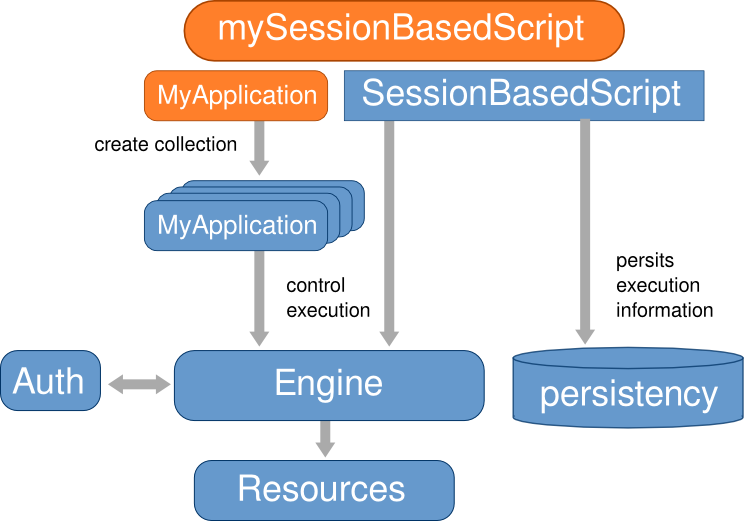
\includegraphics[width=0.8\textwidth]{fig/GC3Pie_execution_model}
\end{frame}

\begin{frame}
  \frametitle{GC3Pie Execution model}
  \begin{columns}
    \column{0.5\textwidth}
      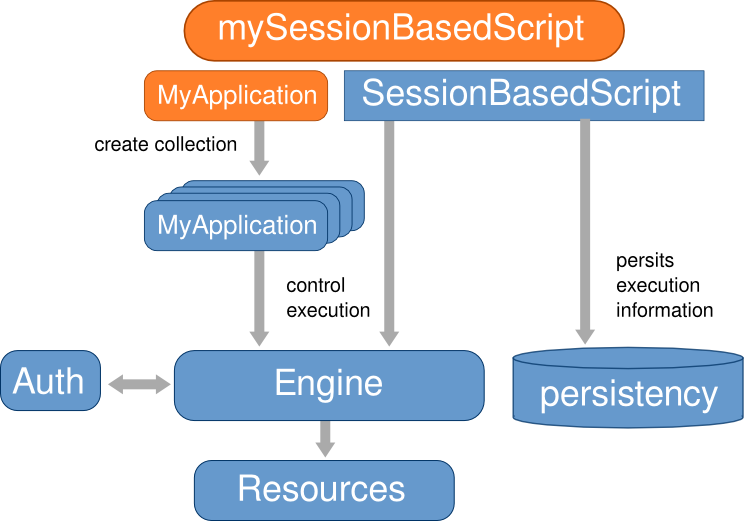
\includegraphics[width=1\textwidth]{fig/GC3Pie_execution_model}
    \column{0.6\textwidth}
  \begin{block}{}
    An application is a subclass of the \texttt{gc3libs.Application}
    class. \\
  \end{block}

  \begin{block}{}
    Applications can be grouped in {\color{Blue}collections}
  \end{block}
  \end{columns}
\end{frame}
  
\begin{frame}
  \frametitle{GC3Pie Execution model}
  \begin{columns}
    \column{0.5\textwidth}
      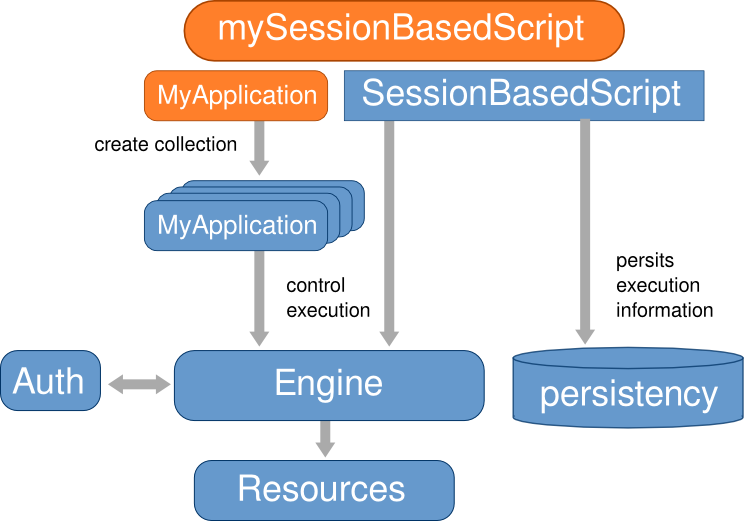
\includegraphics[width=1\textwidth]{fig/GC3Pie_execution_model}
    \column{0.6\textwidth}
  \begin{block}{}
    Execution of collections is delegated to an \texttt{Engine}.\\
    (two modes supported: {\color{Blue}synchronous} and {\color{Blue}asynchronous})
  \end{block}

  \begin{block}{}
    Execution Engine handles the access to computational {\color{Blue}resources}
    (also verifying the proper {\color{Blue}authentication} mechanism)
  \end{block}
  \end{columns}
\end{frame}

\begin{frame}
  \frametitle{GC3Pie Execution model}
  \begin{columns}
    \column{0.5\textwidth}
      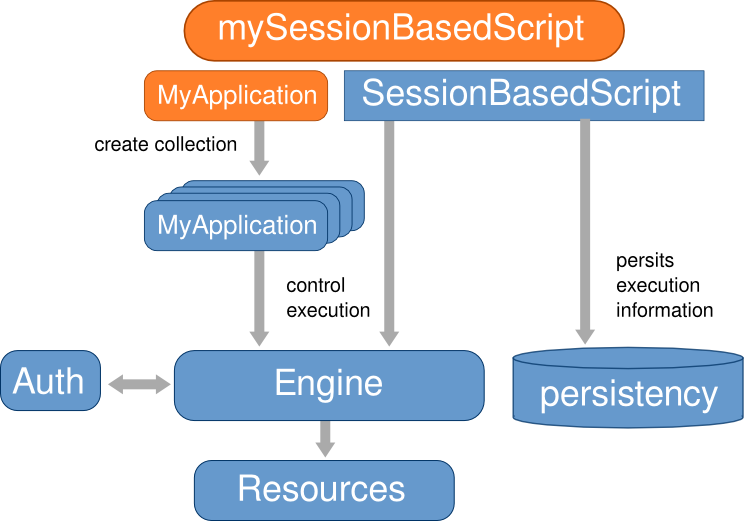
\includegraphics[width=1\textwidth]{fig/GC3Pie_execution_model}
    \column{0.6\textwidth}
  \begin{block}{}
    A convenient class {\color{Blue}SessionBasedScript} contains already
    most of the control logic for instructing the execution engine
  \end{block}

  \begin{block}{}
    \texttt{SessionBasedScript} takes also care of {\color{Blue}persisting}
    execution information
  \end{block}
  \end{columns}
\end{frame}


\begin{frame}
  \frametitle{A simple high-throughput script structure\ldots{}}
  
  \begin{enumerate}
  \item Initialize computational resource (e.g., authentication step)
  \item Prepare files for submission
  \item Submit jobs
  \item Monitor job status (loop)
  \item React on failures (e.g. resubmit)
  \item Retrieve results
  \item Postprocess and display
  \end{enumerate}
\end{frame}

\begin{frame}
  \frametitle{A high-throughput script with GC3Pie, revisited}
  
  \begin{enumerate}
  \item \emph{Create a gc3libs.core.Core instance}
  \item \emph{Create a gc3libs.persistence.FilesystemStore instance}
  \item \emph{Create a gc3libs.core.Engine instance}
  \item \emph{Load saved jobs into it}
  \item Create \emph{new} instance(s) of the application class
  \item \emph{Let engine manage jobs until all are done}
  \item \sout{Retrieve results} (the \texttt{Engine} does it)
  \item Postprocess and display
  \end{enumerate}
  
  Steps 1-4, and 6-7 are automatically done by the
  \texttt{SessionBasedScript} class.
\end{frame}

\begin{frame}
\frametitle{Job dependency management}
  \begin{block}{}
  An \texttt{Engine} manages all jobs concurrently.
  What if there are inter-application dependencies?
  \end{block}

  \begin{block}{}
  GC3Pie provides {\color{Blue}Task composition} support (workflow), created
  programmatically from Python code.
  \end{block}

  \begin{block}{}
  Which means, no graphical editor.  But also means you can create
  workflows {\color{Blue}on-the-fly} as your computation proceeds.
  \end{block}
\end{frame}

\end{document}
